\documentclass{beamer}

\usepackage{minted}
\usepackage{pgf}
\usepackage[utf8]{inputenc}
\usepackage{mdframed}

\BeforeBeginEnvironment{minted}{\begin{mdframed}}
\AfterEndEnvironment{minted}{\end{mdframed}}

\title{Applying \textbf{one} FP Pattern: Monoids}
\subtitle{Original Title: Applying FP Patterns (sorry)}
\author{Markus Hauck}
\date{Scala.IO, 2016}
\subject{Computer Science}

\useinnertheme{default}

\definecolor{MidnightBlue}{RGB}{68,72,169}
\definecolor{Supernova}{RGB}{227,158,0}
\definecolor{MediumSpringGreen}{RGB}{0, 227, 158}
\definecolor{Purple}{RGB}{158,0,227}
\definecolor{ScalaIO}{RGB}{187,0,39}

\definecolor{shadecolor}{RGB}{227,158,0}

\usecolortheme[named=ScalaIO]{structure}

\setbeamercolor{my header}{fg=ScalaIO,bg=black}
\setbeamercolor{my footer}{fg=ScalaIO!90,bg=black}
\setbeamercolor{my footer 2}{fg=ScalaIO!90,bg=black!90}
\setbeamercolor{my page number}{fg=black,bg=ScalaIO!90}

\setbeamercolor{section in head/foot}{fg=white}
\setbeamercolor{mini frame}{fg=ScalaIO}

\setbeamertemplate{headline}{%
  \begin{beamercolorbox}[wd=\paperwidth,ht=5ex,dp=5ex]{my header}
    \insertnavigation{\paperwidth}
  \end{beamercolorbox}
  \begin{pgfpicture}{0mm}{0mm}{0mm}{0mm}
    \pgfsetlinewidth{0.5mm}
    \color{ScalaIO}
    \pgfline{\pgfpoint{0.01\paperwidth}{-1mm}}{\pgfpoint{0.8\paperwidth}{-1mm}}
  \end{pgfpicture}
  \begin{pgfpicture}{0mm}{0mm}{0mm}{0mm}
    \pgfsetlinewidth{0.5mm}
    \color{ScalaIO}
    \pgfline{\pgfpoint{0.0025\paperwidth}{-0.76mm}}{\pgfpoint{0.0025\paperwidth}{-0.07\paperwidth}}
  \end{pgfpicture}
}

\setbeamertemplate{footline}{%
  \hbox{%
  \begin{beamercolorbox}[wd=0.55\paperwidth,ht=2.5ex,dp=1ex]{my footer}
    \hspace{1mm}\insertshortauthor{} - \insertshorttitle{} - codecentric AG
  \end{beamercolorbox}
  \hspace{-2mm}
  \begin{beamercolorbox}[wd=0.40\paperwidth,ht=2.5ex,dp=1ex]{my footer 2}
    \hspace{1mm}\insertsubsection{}
  \end{beamercolorbox}
  \hspace{-2mm}
  \begin{beamercolorbox}[wd=0.06\paperwidth,ht=2.548ex,dp=1.01ex,center]{my page number}
    \insertframenumber{}
  \end{beamercolorbox}
}
  \begin{pgfpicture}{0mm}{0mm}{0mm}{0mm}
    \pgfsetlinewidth{0.5mm}
    \color{ScalaIO}
    \pgfline{\pgfpoint{0.8\paperwidth}{4.5mm}}{\pgfpoint{0.99\paperwidth}{4.5mm}}
  \end{pgfpicture}
  \begin{pgfpicture}{0mm}{0mm}{0mm}{0mm}
    \pgfsetlinewidth{0.5mm}
    \color{ScalaIO}
    \pgfline{\pgfpoint{0.985\paperwidth}{4.255mm}}{\pgfpoint{0.985\paperwidth}{0.1\paperwidth}}
  \end{pgfpicture}
}

\setbeamertemplate{navigation symbols}{}


\setbeamercolor*{block title}{fg=white,bg=black}
\setbeamercolor*{block body}{bg=black!20}

\setbeamercolor*{block title alerted}{use={normal text,alerted text},fg=black,bg=ScalaIO}
\setbeamercolor*{block body alerted}{bg=black,fg=black!20}

\setbeamercolor*{block title example}{fg=black,bg=ScalaIO!90}
\setbeamercolor*{block body example}{bg=black!20}
\setbeamercolor*{example text}{fg=ScalaIO}

\setbeamertemplate{mini frames}[box]
\setbeamersize{mini frame size=3pt}

\setbeamertemplate{blocks}[rounded][shadow=true]

\renewcommand\texttt[1]{\mintinline{scala}/#1/}

\begin{document}
\frame{\titlepage}

\section{Intro}
\label{sec:intro}

\begin{frame}
  \frametitle{Introduction}
  \begin{itemize}
  \item many new useful patterns in FP
  \item today: Monoids
  \item after enlightenment, apply this with Apache Spark
  \end{itemize}
\end{frame}

\section{Composition}

\begin{frame}
  \frametitle{Lego vs Duplo}
  \begin{center}
    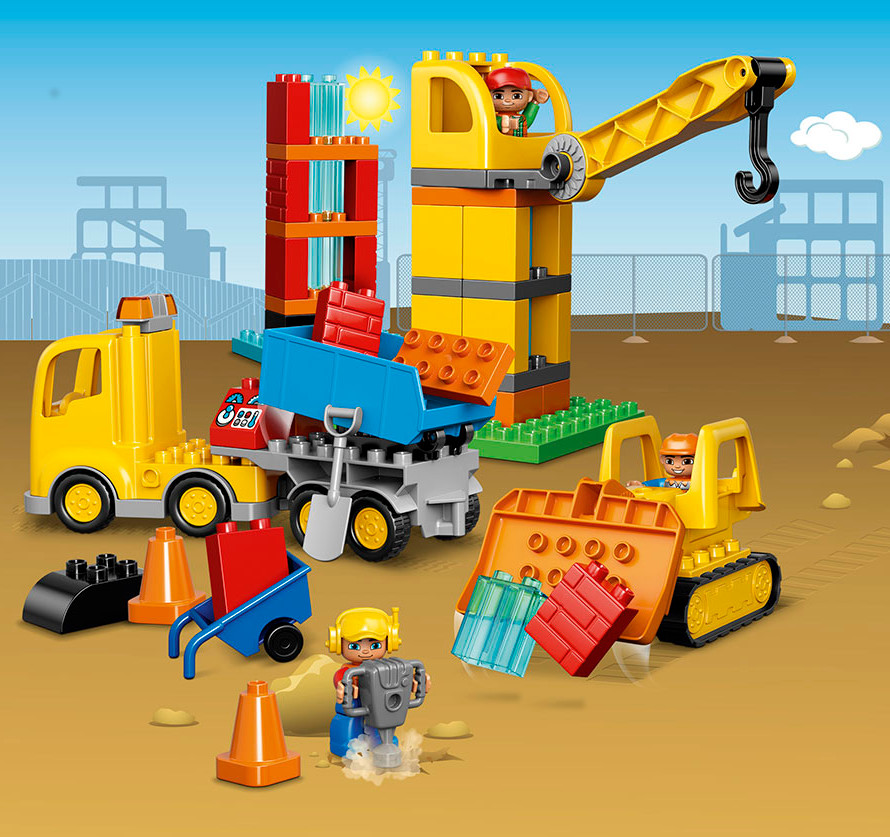
\includegraphics[width=0.45\textwidth]{../images/duplo-construction.jpg}
    \hspace{1mm}
    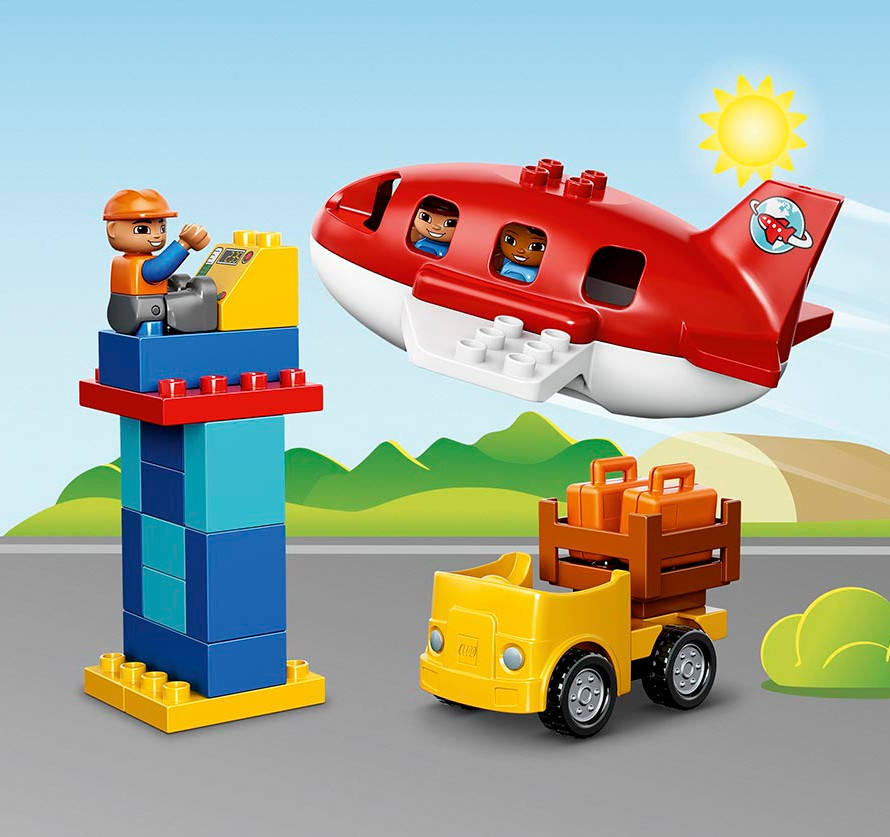
\includegraphics[width=0.45\textwidth]{../images/duplo-airport.jpg}
  \end{center}
  \vfill
  \begin{center}
    {\tiny pictures from \url{shop.lego.com}}
  \end{center}
\end{frame}

\begin{frame}
  \frametitle{Lego vs Duplo}
  \begin{center}
    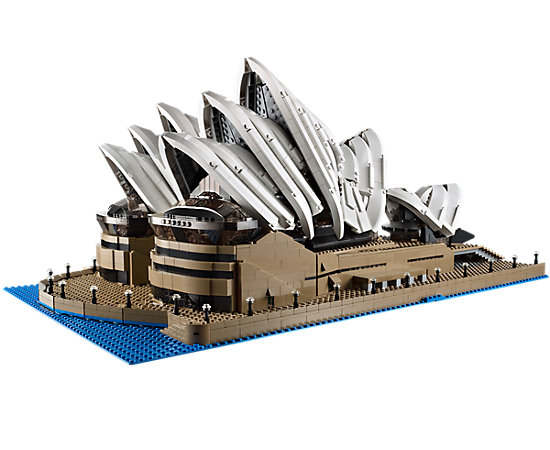
\includegraphics[width=0.45\textwidth]{../images/lego-sydney-opera.jpg}
    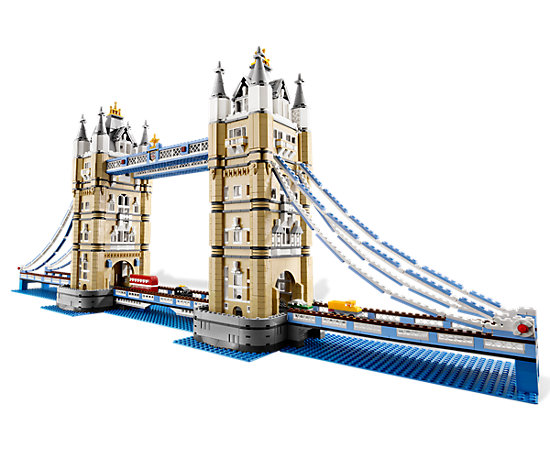
\includegraphics[width=0.45\textwidth]{../images/lego-tower-bridge.jpg}
  \end{center}
  \vfill
  \begin{center}
    {\tiny pictures from \url{shop.lego.com}}
  \end{center}
\end{frame}

\begin{frame}
  \frametitle{Lego vs Duplo}
  \begin{itemize}
  \item Duplo favours specialized building blocks that do
    \textbf{not} compose
  \item therefore very limited reuse, blocks tend to be too big
  \item Lego on the other side focuses on small composable building
    blocks
  \item blocks can conveniently be reused for other purposes
  \item limited use of specialized building blocks
  \item OO tends to be like Duplo, FP tends to be like Lego
  \end{itemize}
\end{frame}

\section{Monoids}

\begin{frame}
  \frametitle{Monoids}
  \begin{itemize}
  \item intuition: ``combine stuff''
  \item you can create values from thin air via \texttt{Monoid.empty}
  \item combine two values via \texttt{Monoid.combine} / \texttt{|+|}
  \end{itemize}
\end{frame}

\begin{frame}[fragile]
  \frametitle{Monoid Laws}
\begin{minted}{scala}
// 1) left identity
empty |+| x === x

// 2) right identity
x |+| empty === x

// 3) associative
x |+| (y |+| z) === (x |+| y) |+| z
\end{minted}
\end{frame}

\begin{frame}[fragile]
  \frametitle{Monoid Typeclass}
\begin{minted}{scala}
trait Monoid[A] {
  def empty: A
  def combine(lhs: A, rhs: A): A
}

implicit val intPlus: Monoid[Int] = {
  new Monoid[Int] {
    def empty: Int = 0
    def combine(lhs: Int, rhs: Int): Int =
      lhs + rhs
  }
}
\end{minted}
\end{frame}

\begin{frame}
  \frametitle{More Monoids}
  \begin{itemize}
  \item Numeric types with addition / multiplication / min / max
  \item \texttt{List}/\texttt{Vector}/\texttt{Set}
  \item lots of others...
  \item more important: composes nicely like legos
  \end{itemize}
\end{frame}

\begin{frame}[fragile,fragile]
  \frametitle{Monoids Compose (Lego Principle)}
  \begin{tabular}{l l}
    \texttt{Map[A,B]} & if \texttt{B} is a \texttt{Monoid} \\
    \texttt{A => B} & if \texttt{B} is a \texttt{Monoid} \\
    \texttt{Future[A]} & if \texttt{A} is a \texttt{Monoid} \\
    \texttt{(A,B)} & if \texttt{A} \textbf{and} \texttt{B} are \texttt{Monoid}s
  \end{tabular}

\begin{minted}{scala}
val m1 = Map("as" -> 21, "bs" -> 4)
val m2 = Map("as" -> 21, "cs" -> 2)
m1 |+| m2
//  Map("as" -> 42, "bs" -> 4, "cs" -> 2)
\end{minted}
\end{frame}

\begin{frame}[fragile]
  \frametitle{Composition Demo}
  \onslide<1>
\begin{minted}{scala}
Config => A
\end{minted}
  \onslide<2>
\begin{minted}{scala}
Config => Future[A]
\end{minted}
  \onslide<3>
\begin{minted}{scala}
Config => Future[Map[String,A]]
\end{minted}
  \onslide<4>
\begin{minted}{scala}
Config => Future[Map[String,(A,B)]]
\end{minted}
  \onslide<5>
\begin{minted}{scala}
Config => Future[Map[String,(A,Option[B])]]
\end{minted}
\end{frame}

\section{Apache Spark}

\begin{frame}
  \begin{center}
    
\includegraphics[width=0.6\textwidth]{../images/disapproval.jpg}
  \end{center}
  \begin{center}
    {\large I thought this was about \textbf{applying} patterns!}
  \end{center}
\end{frame}

\begin{frame}
  \frametitle{Apache Spark}
  \begin{itemize}
  \item Apache Spark:
    \begin{itemize}
    \item analysis of a text (huuuuge)
    \item run in cluster
    \end{itemize}
  \item some possible metrics over text
    \begin{itemize}
    \item word count
    \item char count
    \item min/max word length
    \item avg word length
    \item \dots (be flexible)
    \end{itemize}
  \item \textbf{goal}: single traversal $\leftrightarrow$ \textbf{easy} composition
  \end{itemize}
\end{frame}

\begin{frame}[fragile]
  \frametitle{RDDs and Folds}
\begin{minted}{scala}
abstract class RDD[T] {
  /**
   * Aggregate the elements of each partition,
   * and then the results for all the partitions,
   * using a given associative function and a
   * neutral "zero value".
   */
  def fold(zeroValue: T)(op: (T, T) => T): T
}
\end{minted}
\end{frame}

\begin{frame}[fragile]
  \frametitle{Monoidal RDDs}
\begin{minted}{scala}
implicit class MonoidRDD[T](val rdd: RDD[T])
  extends AnyVal {

  // avoid conflicts with fold/reduce etc
  def combine(implicit M: Monoid[T]): T =
    rdd.fold(M.empty)(M.combine(_,_))

}
\end{minted}
\end{frame}

\begin{frame}[fragile,fragile]
  \frametitle{The Program}
\begin{minted}{scala}
val file = "/some/file.txt"
val sc: SparkContext = new SparkContext(conf)
val words = sc.textFile(file).flatMap(_.split("""\s+"""))
val wordMonoids = words.map(expand)

val z = Monoid.empty[(Option[Max[Int]],Option[Min[Int]],Int,Int)]

def expand(word: String) = {
  (Option(Max(word.length)), Option(Min(word.length)), word.length, 1)
}

val (max,min,chars,words) = wordMonoids.fold(z)(_ |+| _)
\end{minted}
\end{frame}

\begin{frame}[fragile]
  \frametitle{Running this program}
\begin{minted}{text}
Scala.io - The Scala event in France
\end{minted}

\begin{minted}{scala}
Seq("Scala.io","The","Scala","event","in","France")
\end{minted}

\begin{minted}{scala}
Seq(
  (Some(Max(8)),Some(Min(8)),8,1), // Scala.io
  (Some(Max(3)),Some(Min(3)),3,1), // the
  (Some(Max(6)),Some(Min(6)),6,1), // Scala
  // ...
)
\end{minted}

\begin{minted}{scala}
(Some(Max(8)),Some(Min(3)),17,3)
\end{minted}

\end{frame}

\begin{frame}
  \frametitle{Easy Extension}

\end{frame}

\section{Almost Done}

\begin{frame}
  \frametitle{More Monoid Tricks}
  \begin{itemize}
  \item ``filter'' values via \texttt{mempty} value
  \item map + reduce == two phase computation via monoids
  \item finger trees, implement multiple data structures using monoids
  \item drawing diagrams (haskell)
  \end{itemize}
\end{frame}

\end{document}
